\chapter{Initiation into Geometry}

\begin{center}
{\em By}~ H. FREUDENTHAL
\end{center}

\blfootnote{This address was given at the South Asian Conference on Mathematical Education held on 22-28 February 1956 at the Tata Institute of Fundamental Research, Bombay.}
\setcounter{pageoriginal}{82}
Why\pageoriginale do we teach geometry ? This is a question we have discussed for long years in the work group for mathematics of the Netherlands' section (W.V.O.) of the New Education Fellowship. Young nations have the liberty to construct an educational system of their own. The old countries are locked up in their own traditions as in a prison. Teaching programs are the main strong-holds of conservative education. Modern educators who wish to avoid falling in the grooves of tradition, should re-examine the program, again and again, in details as well as on the whole.

\smallskip
In the years 1948-1952, we tried to draw up a new program for secondary instruction of mathematics. There has been a strong tendency towards fixation in Dutch mathematical education. When our work was finished, we had cancelled many traditional topics, and in return we had added a few new ones. But when we began, we hunted for a criterion, for general rules, in order to know whether a topic should be admitted or rejected. Mathematics has proved to be of immense use for both society and the individual. Utility is a mighty touchstone. A program that can stand all tests of usefulness looks like a mathematically proved theory.

\smallskip
For a long time people stuck to the formal value of mathematical education. But formal training is a dangerous argument. It is easy to justify the most old fashioned topics by formal reasons. However, stepping on through algebra, trigonometry, analytic geometry, calculus, we did not detect any aim of formal education that could not be realized within the range of a program which had been determined only by the test of usefulness.

\smallskip
There is one exception : Euclidean geometry. A pragmatical program of geometry could be confined to an extremely small group\pageoriginale of theorems (like the Pythagorean theorem), some evident properties of similar figures, and a few formulas for circumferences, areas and volumes. Pragmatism does not call for any logical system of geometry like that granted us by the Euclidean tradition. We never thought however of abolishing geometry as an object of teaching.

\smallskip
Anxious to avoid vague formal arguments, we did not succeed in 1952 in unearthing the roots of our faith in geometrical instruction. Today after long years of discussion, we might better accomplish this task. I believe today we should state :

\smallskip
Geometry, as a logical system, is a means---and even the most powerful means---to make children feel the strength of the human spirit, that is : of their own spirit.

\smallskip
If this is really our goal, teaching geometry is an unparalleled strife between ideal and realization. I do not know whether a child engaged in his mathematical problems ever reached the conclusion that mathematics has been the work of outstanding human geniuses, but in any case, I am pretty sure that mathematics is rather a means to convince children of their own mental inferiority, not only in Holland, but all over the world.

\smallskip
In our country teaching algebra and geometry starts in the first form of the secondary educational system, that is to children aged 12 years and over. Mostly this school geometry is a watered Euclid in spite of the general conviction that children are not mature for logical rigidity at this age. This maturity must be not the pre-supposition, but the preliminary aim of the first geometrical teaching. As there are children who never reach it, there would be little sense in teasing those pupils with Euclid. There is a simple test whether the level of maturity for the geometrical system has been reached : firstly, the child must have discovered the fact of the enchantment of geometrical truth, secondly, it must have grasped the necessity of this enchantment, and thirdly, it must have been seized by this idea in such a measure that it longs seriously to proceed along the lines of the logical system.

There\pageoriginale are many ways of initiation to geometry. The most outstanding example is the ``{\em Ubungensammlung}'' (1931) of Mrs. T. Ehrenfest-Afanassjewa, who still joins the work of our study group in spite of her great age. As a whole Mrs. Ehrenfest's system has never been practically tried out, but nevertheless it has greatly influenced Dutch geometrical education.

To quote another example : Emma Castelnuovo's well-known ``{\em Geometria Intuitiva}'' of 1948.

I will not treat these methods, which can be easily approached by all persons interested in educational problems. Likewise, I will not occupy myself with courses which still show stronger or weaker relations to classical geometrical text-books. I shall confine myself to the most striking examples of new approach to the problems of mathematical education, experimentally tested by Dutch teachers.

The first method I shall deal with is that of the text-books of Dr. W. J. Bos and P. E. Lepoeter, ``{\em Wegwijzer in de Meetkunde''}. It is the most unusual and the most remarkable course of school geometry I every saw. I do not know any mathematical text-book where every detail has been thought out as deliberately as in the books of Bos and Lepoeter. The greatest pedagogical care has been bestowed on the step-by-step developing of the logical faculties of the pupil. The logical patterns are trained, not as abstractions, but always as structure properties of intuitive data. My exposition will become clearer, if I show you some pages from that text-book.

On the first page, which I reproduce (Fig.~\ref{chap6-fig1}), you see a dozen problems without any text. The pupil will find all data in the figure and the question mark will tell him which angle is to be calculated. You see the pattern to be practised is that of finding out an angle by subtracting a given angle or the sum of given angles from $180^{\circ}$ or $360^{\circ}$ or from another given angle. The pupil shall reason in concreto; afterwards he shall put the way of reasoning in a highly schematized but nevertheless figurative symbolism, a figure as it were of the process of reasoning (Fig.~\ref{chap6-fig2}). Words are avoided as long as possible, large use is made of the implication arrow as a notation symbol. Here\pageoriginale you see a few reasoning patterns, which actually will appear in more or less entangled combinations.

In order to give an impression of the way in which the method develops from the most simple to the more intricate problems, I show you a series of pages (Fig.~\ref{chap6-fig3}-\ref{chap6-fig5}) from the book. You see that equal lines are marked by strokes, parallels by V's, equal angles by dots or arcs, right angles by a square. (Compare, e.g. Number 39 with 48.) In order to find the angle $D$, the pupil must calculate angle $B$ from the isosceles triangle $ABC$. Number 57 is even more involved. The pupil will try to calculate $Q$ by means of the angles $C$ and $D$; a new difficulty arises from the fact that only the sum of $C$ and $D$ can be known (but no more is wanted). Everybody knows that it is very difficult for a young child to develop or even to follow a composite reasoning. The ability of doing this is trained in the text-book in a thorough way. Auxiliary lines, the night-mares of geometry, are never used. Every problem can be solved by scrutinizing its data. One of the last pages of the book will give you an impression of the level the children will reach after a year. You will notice that highly complicated problems can be solved.

{\parfillskip=0pt After having praised this method, I may raise some objections. Firstly, the lack of motivation. The child is assigned the duty of calculating an angle or proving the equality of two lines, and to put his reasonings in a fixed scheme, but never is he given the opportunity to ask why he must do so. Motivated education will encourage children to raise problems, and to formulate them, and it will stimulate the desire of solving the problems which have emerged. I fear that this method does not give enough room to this activity. Secondly, the method is too rigid. Though it is written for individual and group instruction, there is littel liberty. Thirdly, most of the problems are not interesting, they have too little hold over the children, and they will not stimulate their imagination. Fourthly, I think that the systematical training of logical patterns is started too early. It may be a fault to impose an algorithm on children before they vividly feel the need of it. But in spite of these \par}

\newpage

~\phantom{a}
\vfill

\begin{figure}[H]
\centering
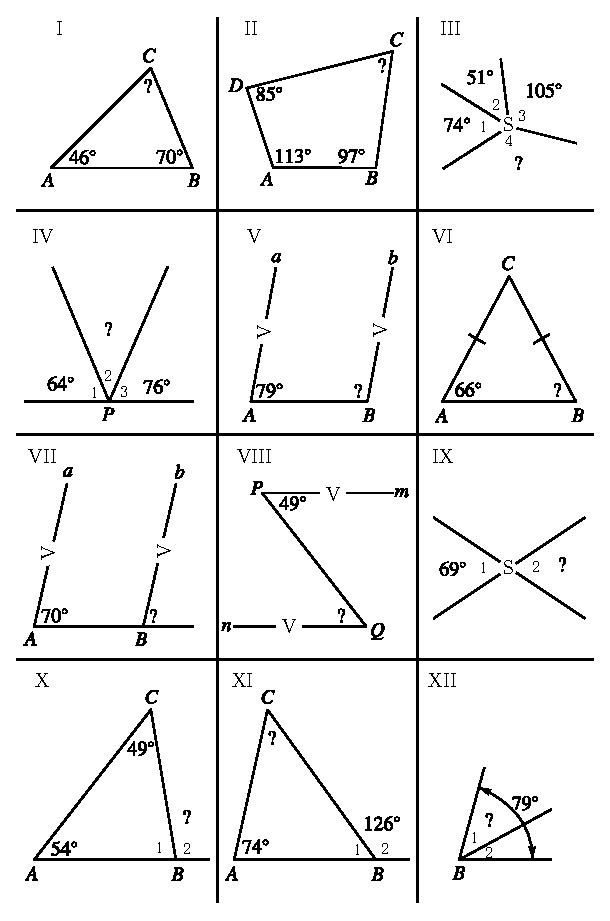
\includegraphics[scale=.95]{figure/fig_01.eps}
\caption{}\label{chap6-fig1}
\end{figure}
\vfill\eject

~\phantom{a}

\vfill
\begin{figure}[H]
\centering
{%\fontsize{9pt}{11pt}\selectfont
\begin{align*}
& keten\text{-}type : 
\left.\begin{array}{l}
a= b\\[3pt]
b=c\\[3pt]
c=d
\end{array}\right\}
\to a=d =\quad(\text{taak~ }21)\\[.5cm]
& aanunllings\text{-}type: 
\left.\begin{array}{l}
a+b=180^{\circ}\\[3pt]
c+d=180^{\circ}\\[3pt]
b=d
\end{array}\right\}
\to a=c\quad(\text{taak~ } 21)\\[.5cm]
& aftrek\text{-}type :
\left.\begin{array}{r@{\;=\;}l}
a+b & c+d\\[3pt]
b & d
\end{array}
\right\} \to a=c \quad (\text{taak~ }21)\\[.5cm]
& optel\text{-}type: 
\left.
\begin{array}{l}
a=b\\[3pt]
c=d
\end{array}\right\}
\to a+c=b+d\quad(\text{taak~ } 21)\\[.5cm]
& balverings\text{-}type:
\left.
\begin{array}{r@{\;=\;}l}
a+b & c+d\\[3pt]
a & b\\[3pt]
c & d
\end{array}
\right\}
\to a=c\quad(\text{taak~ } 25)\\[.5cm]
& vervangings\text{-}type:
\left.
\begin{array}{l}
a=b+c\\[3pt]
b=c
\end{array}
\right\}
\to a=2b\quad\text{(taak 25)}
\end{align*}}\relax
\caption{}\label{chap6-fig2}
\end{figure}

\vfill\eject

~\phantom{a}

\begin{figure}[H]
\centering
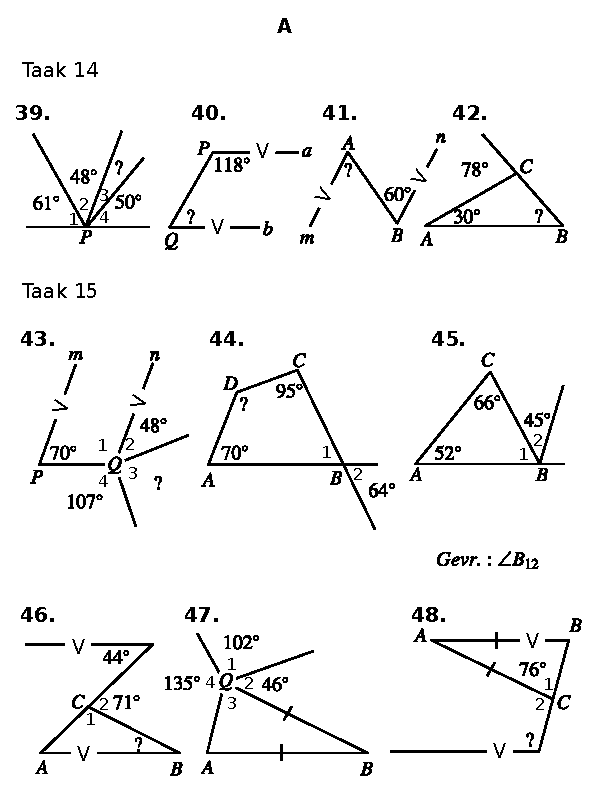
\includegraphics{figure/fig_02.eps}
\caption{}\label{chap6-fig3}
\end{figure}

\vfill\eject

~\phantom{a}

\begin{figure}[H]
\centering
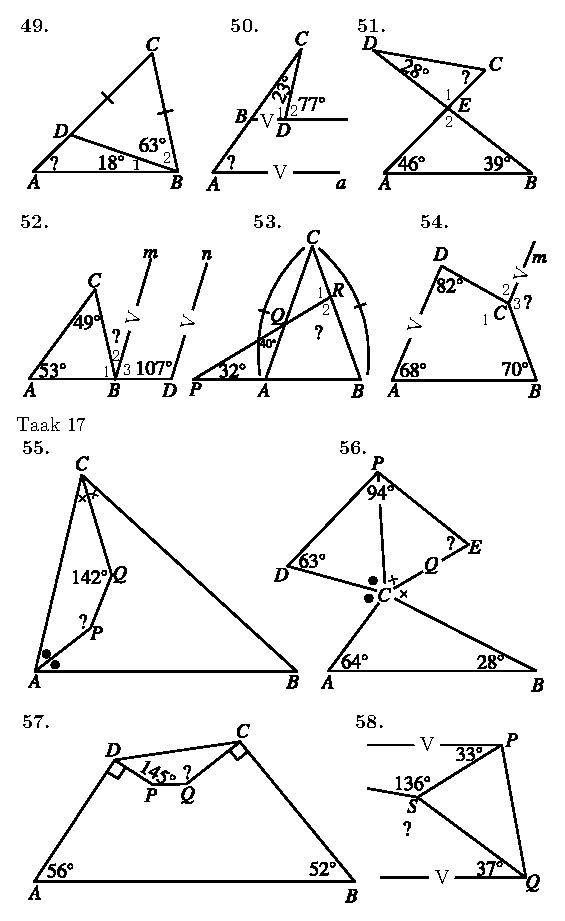
\includegraphics{figure/fig_04.eps}
\caption{}\label{chap6-fig4}
\end{figure}

\vfill\eject

~\phantom{a}

\begin{figure}[H]
\centering
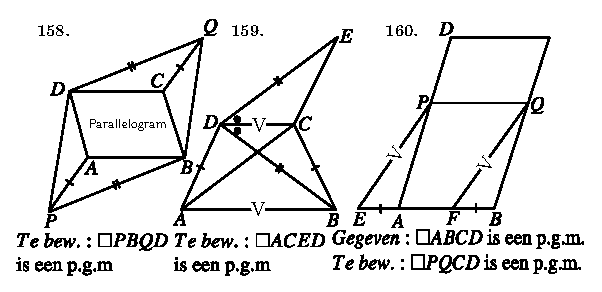
\includegraphics{figure/fig_05a.eps}
\bigskip
\medskip

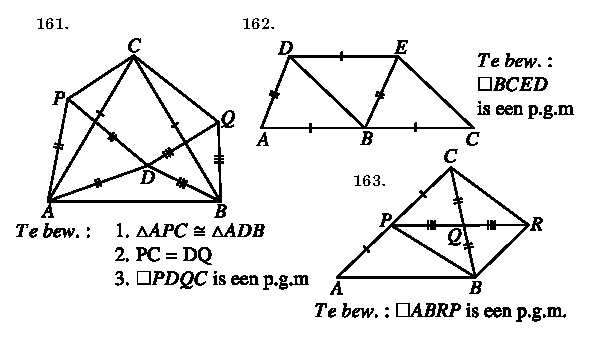
\includegraphics[scale=.95]{figure/fig_05b.eps}

\medskip
\bigskip
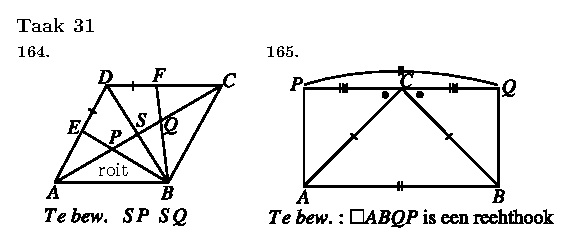
\includegraphics[scale=.95]{figure/fig_05c.eps}
\caption{}\label{chap6-fig5}
\end{figure}

\vfill\eject

~\phantom{a}

\begin{figure}[H]
\centering

\includegraphics{figure/fig_06.eps}
\caption{}\label{chap6-fig6}
\end{figure}

\begin{figure}[H]
\centering
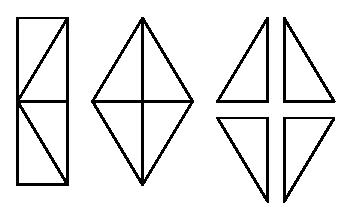
\includegraphics{figure/fig_07.eps}
\caption{}\label{chap6-fig7}
\end{figure}

\begin{figure}[H]
\centering
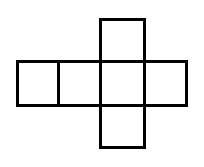
\includegraphics{figure/fig_08.eps}
\caption{}\label{chap6-fig8}
\end{figure}

\vfill\eject

\noindent
\begin{minipage}[b]{4.5cm}
\begin{figure}[H]
\centering
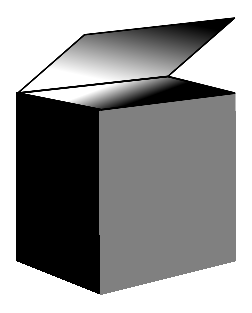
\includegraphics[scale=.9]{figure/fig_09.eps}
\caption{}\label{chap6-fig9}
\end{figure}
\end{minipage}
\qquad
\begin{minipage}[b]{5cm}
\begin{figure}[H]
\centering
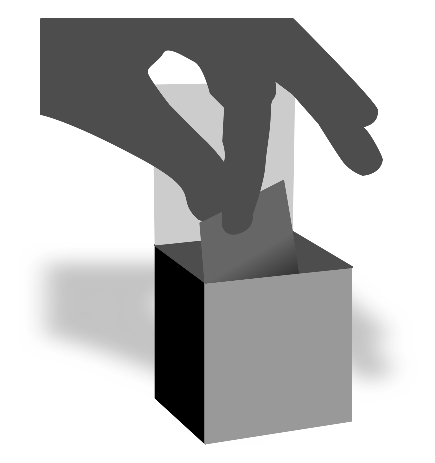
\includegraphics[scale=.9]{figure/fig_10.eps}
\caption{}\label{chap6-fig10}
\end{figure}
\end{minipage}

\vskip 1cm

\begin{minipage}[b]{5.5cm}
\begin{figure}[H]
\centering
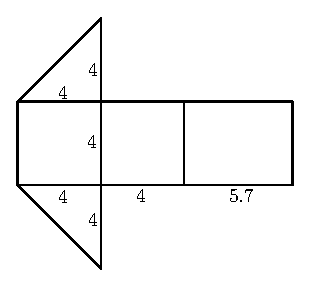
\includegraphics[scale=.9]{figure/fig_11.eps}
\caption{}\label{chap6-fig11}
\end{figure}
\end{minipage}
\qquad
\begin{minipage}[b]{4cm}
\begin{figure}[H]
\centering
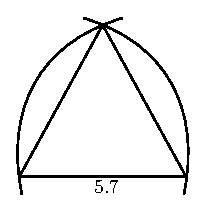
\includegraphics[scale=.9]{figure/fig_12.eps}
\caption{}\label{chap6-fig12}
\end{figure}
\end{minipage}

\begin{figure}[H]
\centering
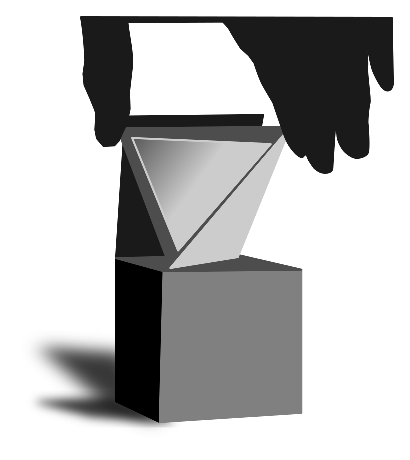
\includegraphics[scale=.9]{figure/fig_13.eps}
\caption{}\label{chap6-fig13}
\end{figure}

\begin{minipage}[b]{5cm}
\begin{figure}[H]
\centering
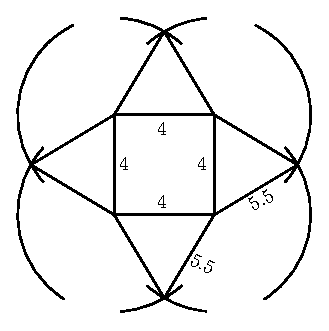
\includegraphics[scale=.9]{figure/fig_14.eps}
\caption{}\label{chap6-fig14}
\end{figure}
\end{minipage}
\quad
\begin{minipage}[b]{5cm}
\begin{figure}[H]
\centering
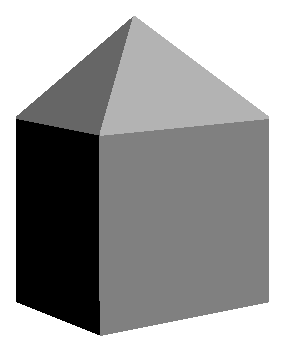
\includegraphics[scale=.9]{figure/fig_15.eps}
\caption{}\label{chap6-fig15}
\end{figure}
\end{minipage}

\begin{figure}[H]
\centering
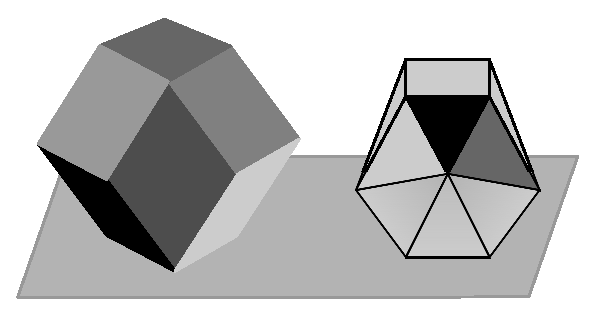
\includegraphics[scale=.9]{figure/fig_16.eps}
\caption{}\label{chap6-fig16}
\end{figure}

\begin{figure}[H]
\centering
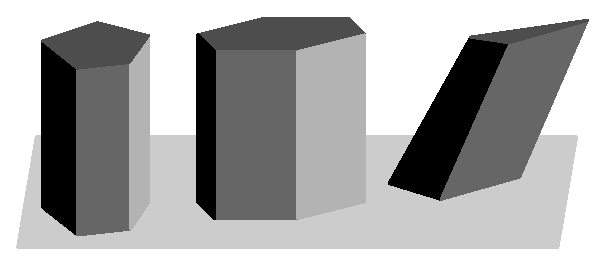
\includegraphics[scale=.9]{figure/fig_17.eps}
\caption{}\label{chap6-fig17}
\end{figure}

\setcounter{pageoriginal}{86}
\noindent
criticisms,\pageoriginale I insist on pointing out the importance of this work, which is not equalled by any other I know.

The viewpoint most antagonistic to this method is supported by a group of teachers, which cannot be plainly characterized by any text-book. The procedures of this group (I may fairly speak of a school of teachers) depend heavily on the use of self-made material of a different kind, cards bearing instructions, models, and construction pieces, like Meccano parts but of a still more flexible structure. 

This movement has originated from two sources. One is the work P. M. van Hiele and his wife, Mrs. D. van Hiele-Geldof. They wrote a series of text-books (Werkboeken) especially for individual and group education, but also used in schools with a class system. In these books the traditional matter of geometrical teaching has been analyzed and arranged under the viewpoint of self-reliance of the pupil. He should not make any appeal to the teacher, until he is hampered by serious difficulyies or he has accomplished a given task. During the initiation to geometry the text-book shall be superseded by the instruction card and other material, developed by the same authors, mainly by Mrs. Dr. van Hiele-Geldof. At the due moment the pupil shall switch over to the text-book.

The other protagonist of this method was Dr. P. J. van Albada, who is now a professor at the University of Indonesia at Bandung. Working independently on the same lines as the van Hieles, he inaugurated an instruction card system, which has been carried on by Dr. Miss J. A. Geldof and Mr. H. J. Jacobs Jr. Interrelations have been established between these two systems.

In Mrs. van Hiele's class-room you will notice a kind of barrow filled with portfolios, each representing a certain task and consisting of a number of instruction cards. The first card of such a portfolio will often contain an instruction, which shall puzzle the child, e.g. a problem that cannot be solved at this level, but no solution of the puzzle will be furnished until the last card of this portfolio will be reached. In any case this last card will lead to a conspicuous piece\pageoriginale of work that may be appreciated by the child as the crown of his labour, and which may awaken the desire of his companions to try the same portfolio.

Let us look at one of the first portfolios, called the rhombo-dodeca\-hedron. (If you protest against terrorizing young children by verbal monstrosities, like rhombo-dodecahedron, I reassure you that in our school geometry almost all Greek and Latin expressions have been push\-ed away by instructive Dutch words, for the greater part invented by Simon Stevin in the beginning of the 17th century. Plain words are of a great advantage in teaching.)

Together with this portfolio the child is given a set of materials : a ruled exercise book, an unruled, one, a sheet of drawing paper, a sheet of thin cardboard, a drawing triangle (set square), a pair of compasses, a ruler-staff, a pair of scissors, a knife, adhesive tape, a box containing models.

The first cards are preparatory. The child learns to erect the perpendicular at a point on a line, to make a right angle by paper-folding, to transfer a line-segment with the aid of compasses, and to draw squares, rectangles, and diagonals. He must say whether the diagonals of a rectangle are equal. He must paste a number of squares of 1 cm$^{2}$ on a rectangular card of 4 cm $\times$ 3 cm, in order to grasp the notion of area. He will lay out a rhomb with four matches, he must say whether he has seen rhombs before, and he must make rhombs by paper-folding. One question is : in how many ways can a rhomb be doubled by folding~? (Fig.~\ref{chap6-fig6}). The child is given four congruent right-angles triangles; he must compose them to get rectangles and to get a rhomb (Fig.~\ref{chap6-fig7}). Which is the area of the rhomb ?

From the sixth upwards I will show you the cards in literal translation.

\smallskip
Sixth card  The cube.
\begin{itemize}
\item[a.] Ask me for a cube (orange model). By how many squares is it bounded ?

\item[b.] How\pageoriginale many square centimeters are needed to paste over the cube ?
\end{itemize}

Measure beforehand the edge of the cube.
\begin{itemize}
\item[c.] Make the adjacent figure (Fig.~\ref{chap6-fig8}) from drawing-paper, but as increased as to get squares with a side of 4 cm. Fold this figure so as to get a cube. (Groove the folding lines beforehand). Do not shut the upper surface (Fig.~\ref{chap6-fig9}).

\item[d.] In the box belonging to this portfolio you will find a lot of cubes with an edge of 1 cm. They are called cubic centimeters. (cm $^{3}$). Build a cube with an edge of 3 cm from those cubes. How many do you need ? Show me what you have done. We will say : The volume of a cube with edge 3 cm is 27 cm$^{3}$.

\item[e.] Which is the volume of the cubes of numbers 6c and 6a ?
\end{itemize}

\newpage

Seventh card : The prism.

\begin{itemize}
\item[a.] Make a rectangle of 5.7 cm $\times$ 4 cm. It fits into the cube you have made in number 6c, in such a way that the cube is divided in two equal parts by this partition wall (Fig.~\ref{chap6-fig10}). Every part will be called a prism.

\item[b.] Draw the figure on drawing-paper (Fig.~\ref{chap6-fig11}). It consists of two squares with a side of 4 cm, a rectangle of 4 cm $\times$ 5.7 cm and two triangles. This figure is called the reticulation of the prism of 7a, because it can be folded so as to get this prism. Cut it out, groove the folding lines, and make the prism.

\item[c.] How many cm$^{3}$
\end{itemize}

Eighth Card :? The tetrahedron.
\begin{itemize}
\item[a.] A cube is also called a hexahedron. Why ? There is also a tetrahedron. It is bounded by four triangles. Draw a triangle with ruler and compasses like that in the adjacent figure (Fig.~\ref{chap6-fig12}).

\item[b.] Draw a figure that may be folded in such a way that you get a tetrahedron with an edge of 5.7 cm. (If you do not succeed, look at the orange model number...). Show me the figure before cutting it out.

\item[c.] Cut\pageoriginale out the reticulation, groove the folding lines, and make a tetrahedron of it.

\item[d.] This tetrahedron can be put in the cube of 6c, so that the lid can be shut. Try it.
\end{itemize}

[Note for the reader : This is just one of the two tetrahedra formed by six surface diagonals of the cube (Fig.~\ref{chap6-fig13}).]

Ninth Card : The pyramid. (Orange models 5, 6, 7.)

The adjacent figure is the reticulation of a pyramid (Fig.~\ref{chap6-fig14}). The side of the square is 4 cm, and from the corners 3.5 cm have been circled round.
\begin{itemize}
\item[a.] Draw this reticulation and make the pyramid.

(The following tasks will be made by three children together.)

\item[b.] How many of these pyramids are wanted for building a cube ? Make as many as you need, and build a cube as big as that of No. 6c.

\item[c.] How many cm$^{3}$ is the volume of the pyramid ?

\item[d.] Stick fast the cube, and paste one pyramid upon each surface of the cube. It becomes a rhombo-dodecahedron. Can you explain the name ? (Fig.~\ref{chap6-fig15}-\ref{chap6-fig16}).

\item[e.] How many cm$^{3}$ is the volume ?

\item[f.] Ask me for the rhombo-dodecahedron (Orange model No....), and make one from thin cardboard. 
\end{itemize}

Tenth Card :

Learn what follows :
\begin{itemize}
\item[a.] A quadrangle with four equal sides is called a rhomb.

\item[b.] A rhomb can be doubled by folding along its diagonals.

\item[c.] The diagonals of a rhomb form right angles.
\end{itemize}

Answer the questions~:
\begin{itemize}
\item[d.] In how many ways can a square be doubled by folding ?

\item[e.] Can you double a rectangle by folding it along a diagonal ?

\item[f.] Can\pageoriginale you double a rectangle by folding it in another way ? (Make a square and a rectangle.) Tell me !

\item[g.] Ask me for the orange models Nos. 2, 4, 5, 6, 7, 8, 10, 1. (Figs.~\ref{chap6-fig17}-\ref{chap6-fir18}). Tell me the names.
\end{itemize}

Read over this portfolio and your exercise book, and ask me for a test card.

Let us now analyze the most important features of this chapter.
\begin{enumerate}
\item All stress is laid on stereometry, not by pure chance, but intentionally. One may argue that geometry teaching should start with stereometry. Except one example---I shall deal with later on,---there are no striking relations of figures in the plane to start geometry with. All properties of figures in the plane are either too silly (e.g. congruence or parallelism---which cannot cause any questions at this stage) or too sophisticated (e.g. Pythagorean theorem, similarity).

\item Solid bodies are less abstract than plane shapes. The child can grasp them in a literal sense. Stereometry meets the children's creative wishes. Figures are drawn, solids are made.

\item The children become acquainted with space. You know how many children, who were keen in planimetry, get in serious difficulties as soon as stereometry starts. Their intuition and imagination have been irreparably waster by three or four years' exclusive planimetric teaching. It has been established by experience that nobody who has started geometry with space, will meet any serious obstacles, when passing to stereometry in the systematic course.

\item The notions of area and volume have been introduced neither by abstract reasoning nor by bluntly appointing that the area is to be length-times-width, and the volume length-times-width-times-height, but by fitting a number of things into one thing---the only psychologically justified manner to introduce them.

\item Fitting is the leading psychological idea of this portfolio, not only for the definition of area and volume. The edges of a reticulation\pageoriginale {\em match} one another. Two prisms {\em fill} a cube. The partition wall {\em fits} into the cube, and the tetrahedron of the six surface diagonals {\em does likewise}. The six pyramids {\em fill} the cube, and placed upon its surfaces their sides will pair-wise {\em merge} into each other---you can feel it by stroking along the surfaces.

Fitting is a motor sensation. Psychologists can tell you how strongly the motor component of the personality is marked at this age, how important motor apprehension and memory may be.

\item Things fit. Do children ask why ? Apart from a rare exception they do not. All these miracles of our space do not seem to make any impression. But they grind as mill-stones. The highest pedagogical virtue is patience. One day the child will ask why, and there is no use to start systematic geometry before that day has come. Even more : it can really do harm. For we have agreed upon teaching geometry as a means to make children feel the strength of the human spirit---that is of their own spirit---and we should not deprive them of the right to make discoveries of their own. The clue of geometry is the word ``why''. Only joy-killers will deliver the clue previously.

\item The miracles of fitting are to prepare maturity for systematic geometry. But if it has been reached they will not become redundant. They will furnish raw material for geometrical thinking, and they will be tokens of the past, when a higher level will have been reached. This is a necessity in mathematical education. The child shall re-call and re-consider the treasure of old problems and re-examine the old solutions at each new stage. In this way, he will be able to judge his own development and his own progress, by retrospective views, as somebody who turns over the leaves of a photograph album, or as a mountain climber who casts a glance back on the way he has gone.

\item It hardly needs stressing that a portfolio like the one analyzed, though a system of instruction, grants a high measure of liberty to the child that works with it. Modern education endeavours to develop not only rational thinking, but also imagination. Mathematics cannot\pageoriginale do without imagination, nor can mathematical teaching. I hope you have felt the strong appeal to imagination in this method.
\end{enumerate}

Let us come back to more special questions. I announced that there is one way to start intuitive geometric teaching with planimetry. The method I have in view is : paving a floor with tiles. This is an idea of van Albada worked out by van Hieles. The slides I shall show you reproduce partially an elaboration by Dr. de Miranda.

Somewhere in the school building a tiled floor or wall will be found. The children get the task of copying it. They may vary the pattern (Fig.~\ref{chap6-fig19}). There are many ways to pave the plane with square tiles. Somebody will try it with triangles (Fig.~\ref{chap6-fig20}). The others join him. The triangles are varied. Any kind of congruent triangles will do it. Any kind of congruent quadrangles too ? Yes ! (Fig.~\ref{chap6-fig21}). Pioneers will explore the pentagon. But the pentagon is obstinate (Fig.~\ref{chap6-fig22}). It does not work. Four is the upper bound. Is it ? Yes, it is. For five cannot succeed. Are you sure ? If five is bad, six is worse. An interruption : It works though. The lavatory is paved with regular hexagons. Many kinds of hexagons can be used for paving the plane (Fig.~\ref{chap6-fig23}).

Why do some polygons fit, and why don't others ? By round about ways the solution will be approached. If the reason is instinctively felt, it will still be difficult to formulate it. Triangles fit because the sum of their angles is half a turn---180$^{\circ}$ : quadrangles because the sum is a full turn---360$^{\circ}$. Pentagons will have one and a half turn---this is an awkward matter. Hexagons give twice a turn, if I can select two angles that sum up to a full turn, I get a chance.

The leading idea of this series of lessons is once more the property of fitting, now applied to the plane. There is but one problem of fitting in the plane, and that one is paving. This problem has been treated here in an extensive measure.

The theorems about the sum of the angles of a polygon have appeared here in a natural way. Not as theorems, but as important problems.\pageoriginale Not as abstract truth, but as incisive relations, which make fitting possible or impossible. Summing up the angles of a polygon has emerged, not as an arbitrary invention of man, but as a necessity of nature. Even congruence has lost its character of dead abstraction.

There is still another reason to prefer tile-paving to the rhombo-dodecahedron. In the portfolio ``rhombo-dodecahedron'' all things fit. Here there is one bad fellow : the pentagon {\em that refused to act}. With the result, that even the laziest is obliged to ask : why ? The children are not guided along a smooth read of thinking, but plunged into dialectics.

After having laid out a floor of equilateral triangles the children make drawings (Fig.~\ref{chap6-fig24}). A minority proceeds without a fixed plan; the triangles are attached one to another at random. The majority build horizontal strips of triangles. It will be a very rare exception if a child discovers the three systems of parallel lines and performs the construction in an economic way. There is little doubt that the first two groups will not be mature at this moment for systematical geometry.

Let us cast a glance into some other portfolios. One is called ``The right-angled triangle''. It starts with two puzzles. A set square moves between two pins fastened into the paper (Fig.~\ref{chap6-fig25}). Which is the locus described by the vertex of the right angle of the set square ? The child will discover it is half a circle or a whole circle. He may ask why or he may not. In any case no proof shall be given. One proceeds to the second puzzle, the famous problem of Menon's: doubling a square. He will not succeed. Now he is given a great number of isosceles right-angles triangles (with sides 2 cm). Can you make a square from five triangles ? With how many can you ? Write down the sequence of these numbers (Fig.~\ref{chap6-fig26}). Can you guess how it would continue if I should give more triangles ? How big are their areas ? Of which squares can you tell me the length of the sides ? Try again to solve the second puzzle !

\begin{figure}[H]
\centering
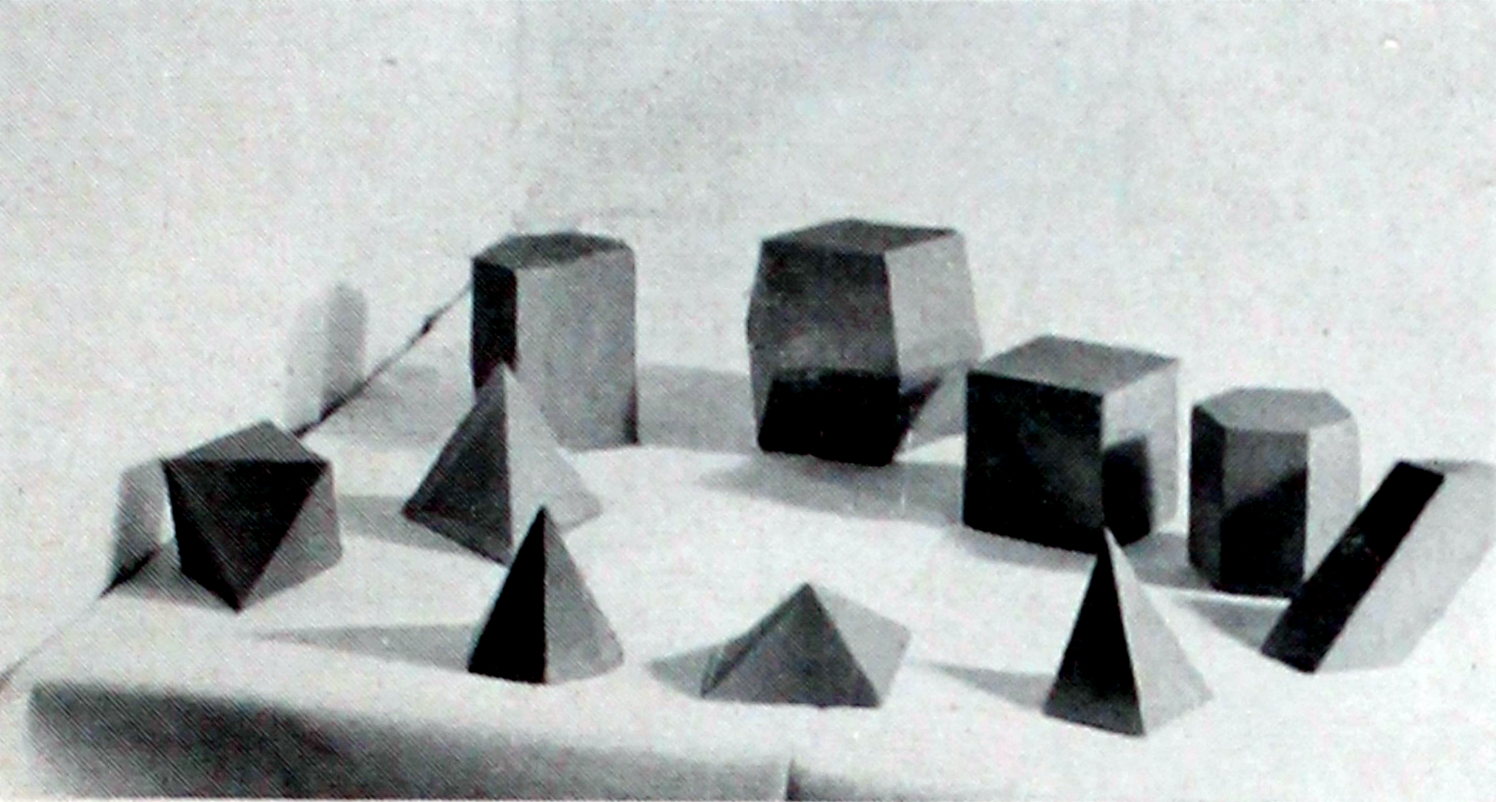
\includegraphics[scale=.9]{figure/fig_18.eps}
\caption{}\label{chap6-fig18}
\end{figure}

\begin{figure}[H]
\centering
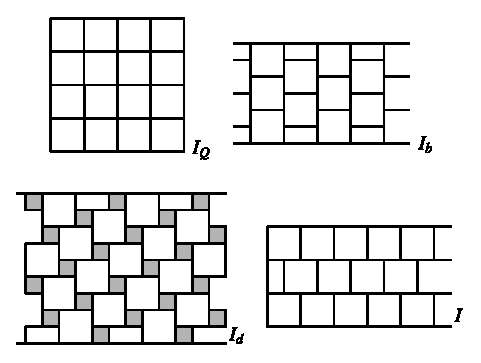
\includegraphics[scale=.9]{figure/fig_19.eps}
\caption{}\label{chap6-fig19}
\end{figure}

\begin{figure}[H]
\centering
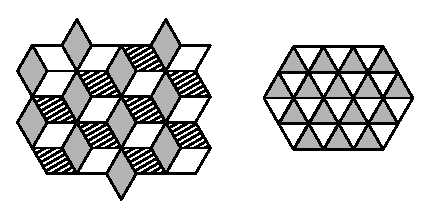
\includegraphics[scale=.9]{figure/fig_20.eps}
\caption{}\label{chap6-fig20}
\end{figure}

\newpage

~\phantom{a}

\vfill

\begin{figure}[H]
\centering
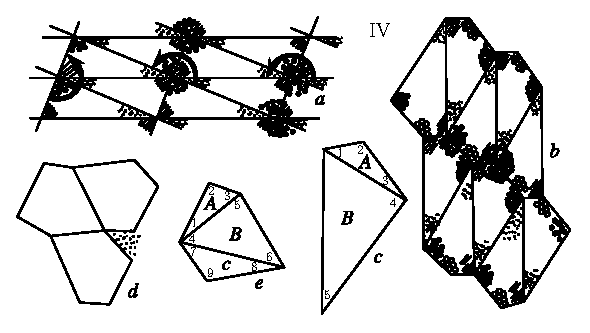
\includegraphics[scale=.95]{figure/fig_21.eps}
\caption{}\label{chap6-fig21}
\end{figure}

\vskip 1cm

\begin{figure}[H]
\centering
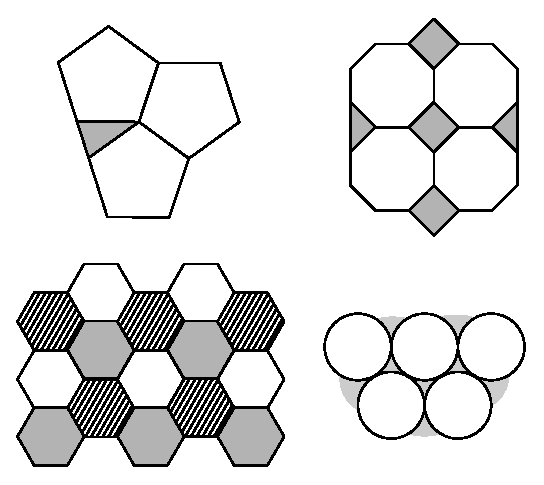
\includegraphics[scale=.95]{figure/fig_22.eps}
\caption{}\label{chap6-fig22}
\end{figure}

\vfill\eject

\begin{figure}[H]
\centering
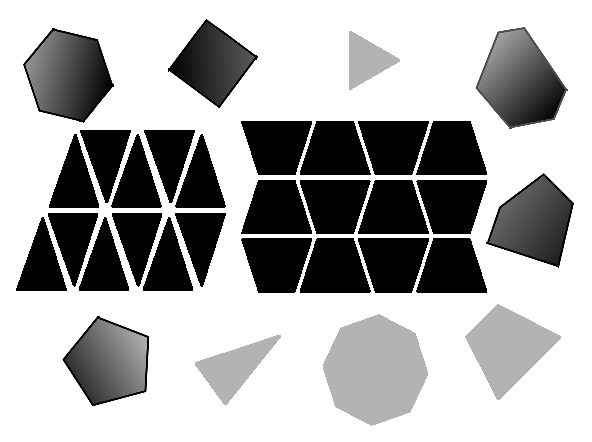
\includegraphics[scale=.9]{figure/fig_23.eps}
\caption{}\label{chap6-fig23}
\end{figure}

\begin{figure}[H]
\centering
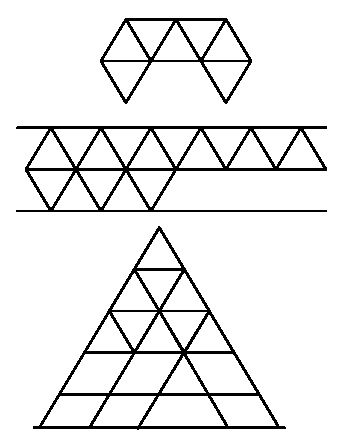
\includegraphics[scale=.9]{figure/fig_24.eps}
\caption{}\label{chap6-fig24}
\end{figure}

\begin{figure}[H]
\centering
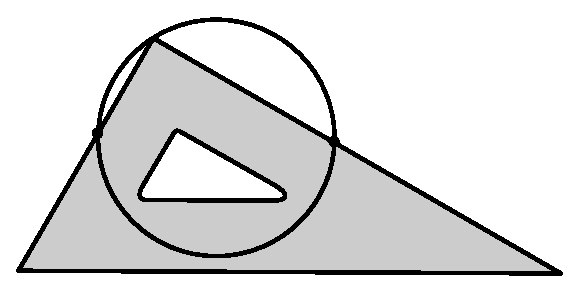
\includegraphics[scale=.9]{figure/fig_25.eps}
\caption{}\label{chap6-fig25}
\end{figure}

\begin{figure}[H]
\centering
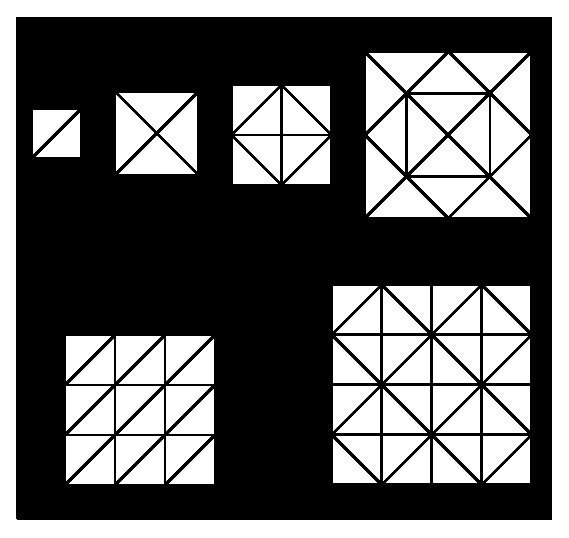
\includegraphics[scale=.9]{figure/fig_26.eps}
\caption{}\label{chap6-fig26}
\end{figure}

\begin{figure}[H]
\centering
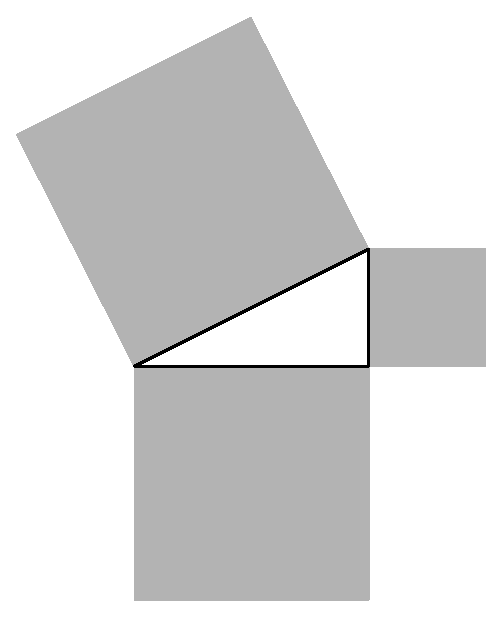
\includegraphics[scale=.9]{figure/fig_27.eps}
\caption{}\label{chap6-fig27}
\end{figure}

\begin{figure}[H]
\centering

\includegraphics[scale=.9]{figure/fig_28.eps}
\caption{}\label{chap6-fig28}
\end{figure}

\begin{figure}[H]
\centering
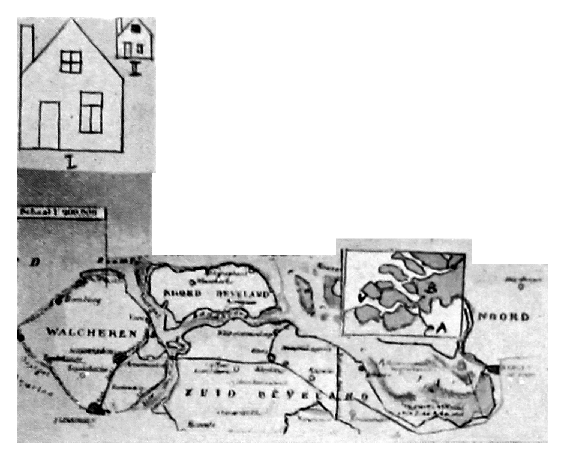
\includegraphics[scale=.8]{figure/fig_29.eps}
\caption{}\label{chap6-fig29}
\end{figure}

\begin{figure}[H]
\centering
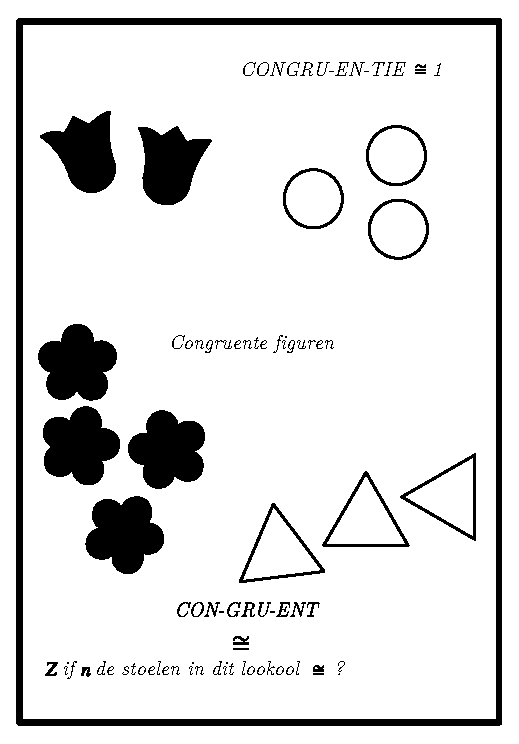
\includegraphics[scale=.7]{figure/fig_30.eps}
\caption{}\label{chap6-fig30}
\end{figure}

\begin{figure}[H]
\centering
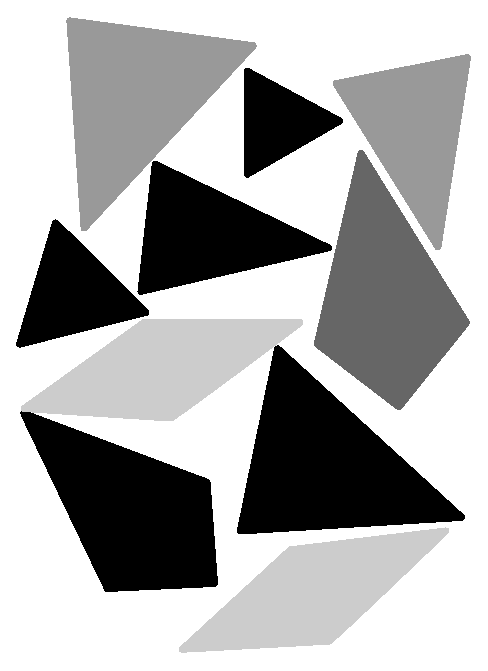
\includegraphics[scale=.7]{figure/fig_31.eps}
\caption{}\label{chap6-fig31}
\end{figure}

\begin{figure}[H]
\centering
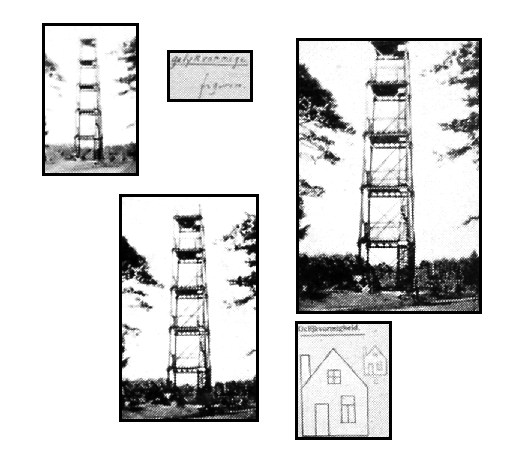
\includegraphics[scale=.8]{figure/fig_32.eps}
\caption{}\label{chap6-fig32}
\end{figure}

\begin{figure}[H]
\centering
\includegraphics[scale=.9]{figure/fig_33.eps}
\caption{}\label{chap6-fig33}
\end{figure}

\begin{figure}[H]
\centering
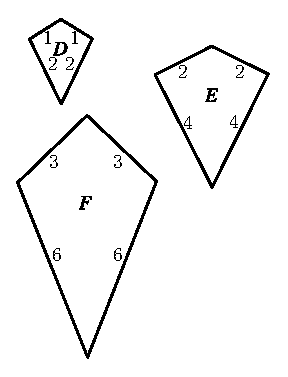
\includegraphics[scale=.9]{figure/fig_34.eps}
\caption{}\label{chap6-fig34}
\end{figure}

\begin{figure}[H]
\centering
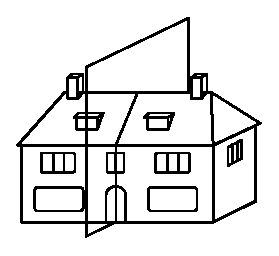
\includegraphics[scale=.9]{figure/fig_35.eps}
\caption{}\label{chap6-fig35}
\end{figure}

\begin{figure}[H]
\centering
\includegraphics[scale=.85]{figure/fig_36.eps}
\caption{}\label{chap6-fig36}
\end{figure}

\begin{figure}[H]
\centering
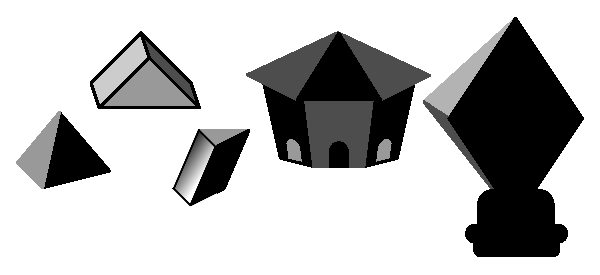
\includegraphics[scale=.85]{figure/fig_37.eps}
\caption{}\label{chap6-fig37}
\end{figure}

\begin{figure}[H]
\centering
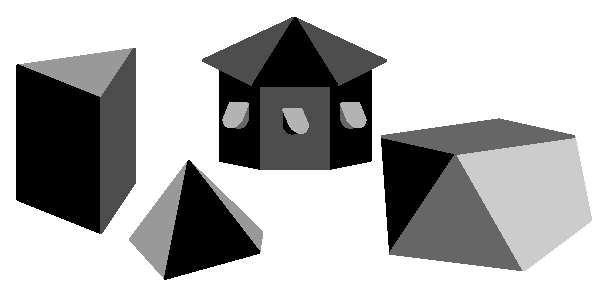
\includegraphics[scale=.8]{figure/fig_38.eps}
\caption{}\label{chap6-fig38}
\end{figure}

\setcounter{pageoriginal}{94}
After\pageoriginale this the child is given a figure that represents Pythagoras' theorem (Fig.~\ref{chap6-fig27}). He is asked to hunt for a proof. He will not succeed. He is given two boxes, which contain respectively the pieces needed to compose the two Figures \ref{chap6-fig28}a and b. Gradually the child will be guided to find the so-called Indian proof of the Pythagorean theorem. As a consequence a lot of theorems about triangles will be developed and the labour will be crowned by the proof of Thales' theorem, the puzzle he started with.

Another portfolio is called : Enlarging and reducing. Similarity is not introduced by a clear cut definition, but by two examples (Fig.~\ref{chap6-fig29}).

Figures such as the two facades are called similar. Look at the two maps of the province Zeeland. The scale of one is 1 : 400,000. How long is the distance from Flushing to Bergen op Zoom ? No scale is mentioned on the second map. Can you determine it ? Let me see it. Determine similarity factor of the two facades.

In the sequel similarity and congruence will be treated in a more systematic manner. Similarity precedes congruence, not by chance, but on good grounds : congruence can be established at sight, whereas similarity puts problems : to determine the similarity factor and to find out criteria of similarity. Likewise similarity of quadrangles and other figures is treated before that of triangles, because the latter case is too special. Indeed, similarity of triangles can be decided by bare arguments about angles, one can dispense with proportionality of sides, and this is a serious disadvantage.

An interesting portfolio treating congruence and similarity is contained in the system of Dr. J. A. Geldof. It proceeds more slowly than that of the van Hieles', but the material defining the fundamental notions is more extensive. I cannot treat this portfolio at full length, but I shall show you the first card (Fig.~\ref{chap6-fig30}) introducing congruence, other material (Fig.~\ref{chap6-fig31}) illustrating it, and one card introducing similarity (Fig.~\ref{chap6-fig32}). This portfolio finishes by a review of solids (Fig.~\ref{chap-fig33}) whre the child is asked to pick out congruent and\pageoriginale similar samples, and by a few questions, partially related to the kits of Fig.~\ref{chap6-fig34}~:

\eject

\begin{itemize}
\itemsep=2pt
\item[a.] The kites $D$ and $E$ are similar. The kites $D$ and $F$ are not similar. Tell me why not ? Take the kites with you.

\item[b.] Draw a kite similar to $F$.

\item[c.] Draw two similar quadrangles.

\item[d.] Can you draw two non-similar quadrangles ? (Orally).

\item[e.] Are circles always similar ?

\item[f.] Are rectangles always similar ?

\item[g.] Mention figures that are always similar.
\end{itemize}

I am sorry I cannot show you van Albada's astonishing material about perspective, which leads the twelve-year olds in a natural way up to fairly complicated designs of descriptive geometry. Van Albada has made the important discovery that the proper place of descriptive geometry in geometrical instruction is not the higher but just the lower level.

As a last example I will draw your attention to one of the most exciting topics which is met in all these systems of initiation into geometry---the phenomenon of symmetry. Ornaments from the dawn of mankind seem to support the thesis that symmetry has been the first geometrical idea that arose in the human mind, and which was given expression in human handicraft. Through an infinity of instances from nature and technics, symmetry may be approached by the childish spirit. It is a remarkable fact that planar symmetry with respect to one axis or a number of axes is a strikingly evident notion whereas many people never really become acquainted with central symmetry, even though they learn mathematics. Few children discover of their own the congruence of the triangles into which a general parallelogram is divided by a diagonal. The only exception are those who have made up parallelograms from triangular tiles and those who have been trained in central symmetry.

Without\pageoriginale further commentary I shall show you some cards and models used in the treatment of symmetry (Fig.~\ref{chap6-fig35}-\ref{chap6-fig38}). It is worth-while mentioning the use made of mirrors as a tool in this chapter.

When drawing my final conclusions I must compare once more the two systems I considered as antagonistic approaches to initial teaching of geometry. The system of Bos and Lepoeter is much more worked out in all details than the other ones. It has been laid down in a textbook accessible to as many teachers as you want, whereas the other methods are confined to comparatively small groups. The first system can be used with real success by any teacher who will make fair attempt to give good instruction. The latter system supposes a depth of psychological background that is not provided by our profoundly scientific, but pedagogically shallow teacher training. In every special case the choice of system (which may be extreme or intermediate) will heavily depend on the teacher's personality structure.

\bigskip
\medskip

{\fontsize{9pt}{11pt}\selectfont Utrecht, Netherlands}\relax



